\documentclass[aspectratio=169,11pt]{beamer}
\usepackage{graphicx,booktabs,xcolor,amsmath,array}
\usetheme{default}
\setbeamertemplate{navigation symbols}{}
\setbeamertemplate{footline}[frame number]
\definecolor{ink}{HTML}{1A202C}
\definecolor{acc}{HTML}{2B6CB0}
\definecolor{warn}{HTML}{C53030}
\definecolor{mut}{HTML}{718096}
\definecolor{soft}{HTML}{EBF4FF}
\setbeamercolor{structure}{fg=acc}
\setbeamercolor{normal text}{fg=ink}
\setbeamerfont{frametitle}{size=\large,series=\bfseries}
\setbeamertemplate{frametitle}{\vspace{6pt}\insertframetitle\par
  \vspace{-4pt}{\color{acc}\rule{\textwidth}{1pt}}}
\setbeamertemplate{itemize item}{\color{acc}\textbullet}
\graphicspath{{../../results/figures/}}
\newcommand{\Hi}[1]{{\color{acc}\textbf{#1}}}
\newcommand{\Bad}[1]{{\color{warn}\textbf{#1}}}

\title{\textbf{How the measurement works}}
\subtitle{From sentences to a number, step by step}
\author{Waiz Khan}
\institute{\small Johns Hopkins University}
\date{\small August 2026}

\begin{document}
{\setbeamertemplate{footline}{}\begin{frame}\titlepage\end{frame}}

% ---------------------------------------------------------------- 1
\begin{frame}{The setup: one grid of sentences}
We take \Hi{300 sentences} and their professional translations into
\Hi{41 languages}. Sentence 7 in German means the same thing as
sentence 7 in Tamil.
\vspace{10pt}

The model reads each one and produces a vector. That gives a grid:
\vspace{6pt}
\begin{center}\small
\begin{tabular}{l|cccc}
 & sentence 1 & sentence 2 & $\cdots$ & sentence 300\\
\hline
English & $h_{1,1}$ & $h_{1,2}$ & & $h_{1,300}$\\
German  & $h_{2,1}$ & $h_{2,2}$ & & $h_{2,300}$\\
$\vdots$ & & & & \\
Tamil   & $h_{41,1}$ & $h_{41,2}$ & & $h_{41,300}$\\
\end{tabular}
\end{center}
\vspace{10pt}
12{,}300 vectors. \Hi{Every question we ask is a question about this
grid.}
\end{frame}

% ---------------------------------------------------------------- 2
\begin{frame}{What the grid actually looks like}
\begin{center}
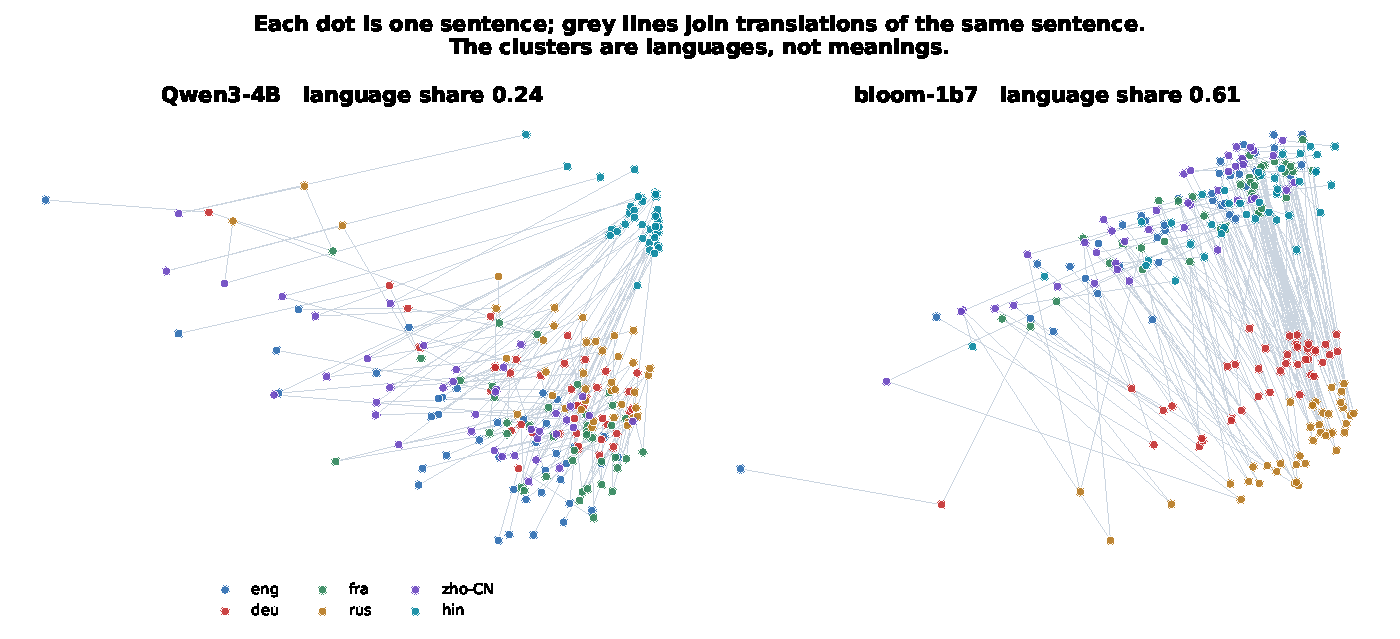
\includegraphics[width=0.86\linewidth]{fig7_geometry.pdf}
\end{center}
\vspace{-6pt}
{\small If the model represented \emph{meaning} and ignored
\emph{language}, every grey line would shrink to a point: all 6
translations of a sentence would land in the same place. Instead the
dots group by colour. \Hi{The model's geometry is organised by language
first.}}
\end{frame}

% ---------------------------------------------------------------- 3
\begin{frame}{Two things move a vector}
Where a vector sits is driven by exactly two systematic factors, plus
noise:
\vspace{8pt}
\[
\underbrace{h_{\ell,c}}_{\text{one cell}} \;=\;
\underbrace{\mu}_{\text{grand average}} +
\underbrace{a_c}_{\substack{\text{which sentence}\\ \text{(meaning)}}} +
\underbrace{b_\ell}_{\substack{\text{which language}\\ \text{(language)}}} +
\underbrace{e_{\ell,c}}_{\text{the rest}}
\]
\vspace{8pt}
\begin{itemize}\setlength\itemsep{5pt}
\item $a_c$ is shared by \emph{all 41 translations} of sentence $c$ ---
it is the column effect
\item $b_\ell$ is shared by \emph{all 300 sentences} in language
$\ell$ --- it is the row effect
\end{itemize}
\vspace{8pt}
{\color{mut}This is a standard two way analysis of variance, applied
per dimension of the representation and then summed.}
\end{frame}

% ---------------------------------------------------------------- 4
\begin{frame}{Separating them: a worked example}
Take one dimension, 2 languages, 3 sentences:
\vspace{4pt}
\begin{center}\small
\begin{tabular}{l|ccc|c}
 & s1 & s2 & s3 & \textbf{row mean}\\
\hline
English & 1.0 & 3.0 & 5.0 & \textbf{3.0}\\
German  & 2.0 & 4.0 & 6.0 & \textbf{4.0}\\
\hline
\textbf{column mean} & \textbf{1.5} & \textbf{3.5} & \textbf{5.5} &
3.5\\
\end{tabular}
\end{center}
\vspace{8pt}
\begin{itemize}\setlength\itemsep{4pt}
\item \Hi{Meaning effects} = column means $-$ grand mean =
$-2,\; 0,\; +2$ \quad(spread out)
\item \Hi{Language effects} = row means $-$ grand mean =
$-0.5,\; +0.5$ \quad(tight)
\item Residual = cell $-$ row $-$ column $+$ grand = $0$ everywhere
\end{itemize}
\vspace{8pt}
Meaning moves these vectors much more than language does. That is a
\Hi{low language share} --- the good case.
\end{frame}

% ---------------------------------------------------------------- 5
\begin{frame}{The number}
\[
\text{language share} \;=\;
\frac{\sigma^2_{\text{language}}}
{\sigma^2_{\text{language}} + \sigma^2_{\text{meaning}}}
\]
\vspace{6pt}
\begin{center}\small
\begin{tabular}{cl}
\toprule
\textbf{0} & language does nothing; all 41 translations of a sentence
land together\\
\textbf{1} & meaning does nothing; all 300 sentences in a language land
together\\
\bottomrule
\end{tabular}
\end{center}
\vspace{12pt}
\begin{itemize}\setlength\itemsep{5pt}
\item Measured across 33 models the value runs from \Hi{0.59 to 0.90}
\item Language identity is the \emph{dominant} organising factor in
every model tested, including the best ones
\item This is the quantity LFS reported, and it is a real and useful
measurement
\end{itemize}
\end{frame}

% ---------------------------------------------------------------- 6
\begin{frame}{It changes with depth, in the same way everywhere}
\begin{columns}[T]
\begin{column}{0.52\textwidth}
\vspace{4pt}
Measured at every layer of 31 models, the shape is always the same:
\vspace{8pt}
\begin{itemize}\setlength\itemsep{5pt}
\item \Hi{high} at the input embedding --- tokens are language specific
\item \Hi{lowest} around the middle to late layers --- the most
language neutral point
\item \Hi{high again} at the output --- the model must commit to words
in one language
\end{itemize}
\vspace{8pt}
What differs between models is \Hi{how deep the dip goes}: 0.38 for
Mistral-Nemo, 0.48 for Llama-3.1, but only 0.87 for Falcon3-3B.
\vspace{6pt}

{\color{mut}All other readings are taken at each model's own minimum.}
\end{column}
\begin{column}{0.48\textwidth}
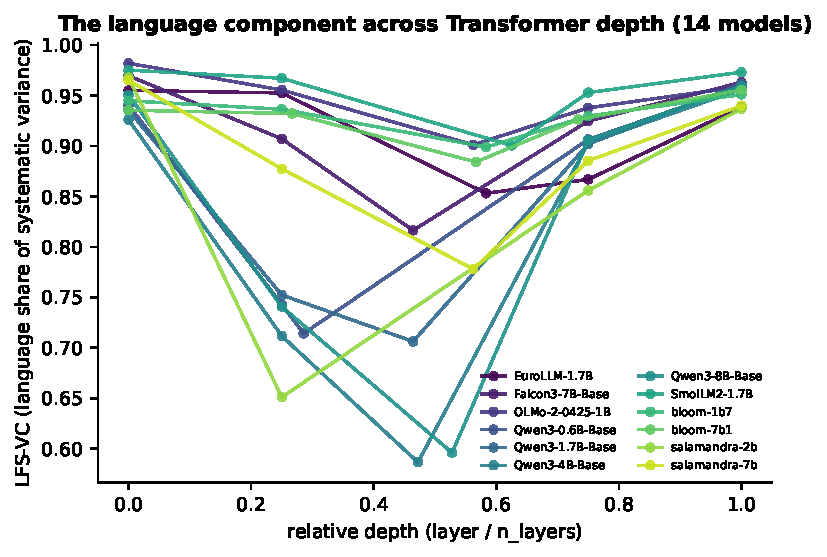
\includegraphics[width=\linewidth]{fig6_layer_profiles.pdf}
\end{column}
\end{columns}
\end{frame}

% ---------------------------------------------------------------- 7
\begin{frame}{Where reporting it as one number goes wrong}
Take the same worked example and \Bad{shrink everything by a factor of
10} --- the model keeps its structure but flattens it:
\vspace{4pt}
\begin{center}\small
\begin{tabular}{l|ccc|c}
 & s1 & s2 & s3 & row mean\\
\hline
English & 0.10 & 0.30 & 0.50 & 0.30\\
German  & 0.20 & 0.40 & 0.60 & 0.40\\
\hline
column mean & 0.15 & 0.35 & 0.55 & 0.35\\
\end{tabular}
\end{center}
\vspace{6pt}
Meaning effects: $-0.2,\,0,\,+0.2$. \quad Language effects:
$-0.05,\,+0.05$.
\vspace{6pt}
\[
\frac{c\,\sigma^2_{\text{language}}}
{c\,\sigma^2_{\text{language}} + c\,\sigma^2_{\text{meaning}}}
\;=\; \text{\Bad{exactly the same number}}
\]
\vspace{2pt}
{\color{mut}Both parts shrank, so the share cannot move. The model lost
almost all its structure and the score is unchanged.}
\end{frame}

% ---------------------------------------------------------------- 8
\begin{frame}{This is not hypothetical}
\Large
A trained variant lost \Bad{95 percent} of its meaning structure at the
measurement layer --- and posted the \Bad{best score in the study}.
\vspace{14pt}

\normalsize
\begin{itemize}\setlength\itemsep{6pt}
\item Confirmed in closed form on controlled distortions: the share
moves less than a millionth while meaning structure falls 99 percent
\item Any measure written as a share of a total inherits this
\item The fix is not a better estimate of the share. It is to
\Hi{report the parts, not the ratio}
\end{itemize}
\end{frame}

% ---------------------------------------------------------------- 9
\begin{frame}{What RMFS reports instead}
Four readings, per language, side by side:
\vspace{10pt}
\begin{enumerate}\setlength\itemsep{7pt}
\item \Hi{Meaning against language} --- the decomposition above,
unchanged. Answers: is the space organised by content or by language?
\item \Hi{Sentence matching} --- for each sentence in language
$\ell$, is its English translation the nearest of the 300 candidates?
Answers: can the model find equivalent content across languages?
\item \Hi{Weakest aligned languages} --- the same matching restricted
to the worst aligned tail. Answers: how bad is it where it is worst?
\item \Hi{Collapse flag} --- meaning structure compared against a
reference checkpoint. Answers: did training destroy structure?
\end{enumerate}
\vspace{8pt}
{\color{mut}The first is a property of the whole grid; the second and
third are properties of individual rows against the English row; the
fourth needs a before and after.}
\end{frame}

% ---------------------------------------------------------------- 10
\begin{frame}{Why four and not one}
\begin{center}
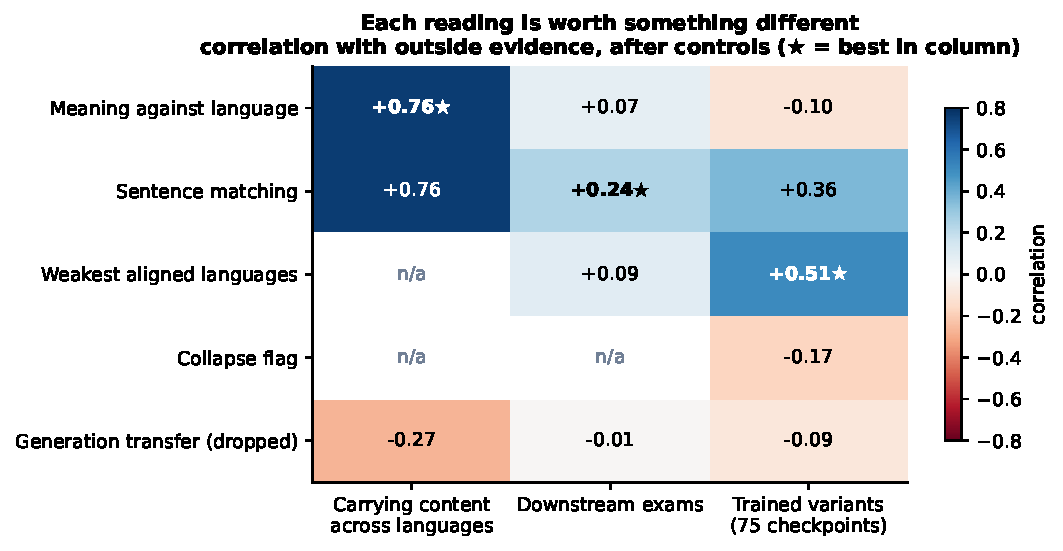
\includegraphics[width=0.78\linewidth]{fig1_validity_matrix.pdf}
\end{center}
\vspace{-4pt}
{\small Each reading was checked against three different kinds of
outside evidence. \Hi{No reading wins two columns.} They measure
genuinely different things, so averaging them into one number throws
away the information that makes them useful.}
\end{frame}

% ---------------------------------------------------------------- 11
\begin{frame}{Turning readings into a score}
Each reading is on its own scale, so they are converted before being
combined:
\vspace{10pt}
\begin{center}\small
\begin{tabular}{ll}
\toprule
1. compute the four readings & per language, at the model's own layer\\
2. convert each to a percentile & against a fixed reference grid of 33
models\\
3. average the four percentiles & giving 0 to 100 per language\\
4. take the median across languages & giving one number per model\\
\bottomrule
\end{tabular}
\end{center}
\vspace{12pt}
\begin{itemize}\setlength\itemsep{4pt}
\item A score of \Hi{74} means better than 74 percent of the reference
models
\item Percentiles rather than raw values, because averaging raw scales
is precisely what let a collapse hide
\item About four GPU minutes per model
\end{itemize}
\end{frame}

% ---------------------------------------------------------------- 12
\begin{frame}{Reading a result}
\begin{center}\small
\begin{tabular}{lcccc}
\toprule
& meaning vs & sentence & weakest & collapse\\
& language & matching & languages & flag\\
\midrule
a healthy model & moderate & high & moderate & 1.0\\
the damaged variant & \emph{moderate} & \emph{high} & moderate &
\Bad{0.05}\\
a poorly aligned model & low & \Bad{low} & \Bad{low} & 1.0\\
\bottomrule
\end{tabular}
\end{center}
\vspace{12pt}
\begin{itemize}\setlength\itemsep{5pt}
\item The damaged variant is invisible on the first three readings and
obvious on the fourth
\item A poorly aligned model is the opposite pattern
\item \Hi{The pattern across the four readings is the diagnosis}; the
single score is only a summary for ranking
\end{itemize}
\end{frame}

\end{document}
